\chapter{Evaluation}
\label{chap:evaluation}

\section{Quantitative evaluation}
\label{sec:quantitative_evaluation}

\subsection{Text extraction}
\label{subsec:text_extraction}

In order to evaluate the quality of the information extracted by the \pextractor{}, 
we decided to compare the genre, century, and the paraphrase-specifc topic to the 
ground truth available for the \dataBlog{}, \dataGutenberg{} and the \dataCustom{} dataset.

We found that the instructions for the \pextractor{} have to be positioned after the text to be extracted, 
due to the inability of the \pextractor{} to return the extracted information in the specified JSON format 
when the prompt was at the beginning of the input for long texts such as those from the \dataGutenberg{} dataset.

\textcolor{red}{TODO: insert table with results}

Irrespective of the quality of the text extraction, we hypothesize that the quality of the final result of the \pgenerator{} will be good irrespective of the quality of the \pextractor{}.
We motivate this by the fact that both the \pextractor{} and the \pgenerator{} are \acp{llm} and therefore generate text similar.
% Attention: Causal vs. masked language model work different

\subsection{Paraphrase generation}
\label{subsec:paraphrase_generation}
To evaluate the quality of the paraphrases generated by the \pgenerator{}, 
we not only computed different paraphrase quality metrics, 
but also compared the text lengths of the generated paraphrases and the original text.

\textcolor{red}{TODO: insert table with results}

% shortcomings of paraphrasing metrics and need for human evaluation
Though easier to reproduce, it is somehow unclear what paraphrase metrics actually measure beyond what their formula states.
While high n-gram overlap might not be the indicator of a good paraphrase in the sense of high syntactic diversity, 
it is not clear if high cosine similarity between the embedding of two texts is a good indicator of a good paraphrase.
Moreover, for all metrics, threshold values for good paraphrases are not well-defined.
It remains to be found whether the worst performing paraphrases are still good enough in terms of human evaluation.
We therefore also employed qualitative evaluation of the paraphrases.

\subsection{Measures and findings}
\label{subsec:measures_and_findings}

% shortcoming of traditional quantitative paraphrase metrics
We used state-of-the art measures for the quantitative evaluation of paraphrases. 
Unfortunately, these measures can be misleading since it is unclear what they actually measure.
Generally high scores in BLEU, ROUGE, METEOR mean nearly identical paraphrase (high n-gram overlap).
In this case, we want value syntactic diversity, rendering these measures unintuitive 
for high values do not necessarily correspond to good paraphrases.
Semantic similarity measurements compare the content of the paraphrase to the original text, 
where the interpretation of the cosine of a vector is not clear either.

% findings
Non-naive paraphrasers generally lower syntactic scores than naive paraphrasers,
supposedly because they have a weaker influence on the \pgenerator{} 
(i.e. disclosing extracted content rather than the original text)
leaving more room for variance in texts.
Consequently, \enquote{bad} scored non-naive paraphrases are good in terms of syntactic diversity.

\section{Qualitative evaluation}
\label{sec:qualitative_evaluation}

In addition to the quantitative evaluation, we qualitatively evaluated the paraphrases generated by the \pgenerator{}.
Prior to the evaluation we specified a list of criteria that a good paraphrase should fulfill.



\subsection{Ablation: Paraphrasing chunks}
\label{subsec:paraphrasing_chunks}

Initially, we hypothesized that smaller chunks of text would lead to better paraphrases, 
since smaller chunks are easer to process and control in terms of topic,
suggesting that the separation of text into smaller chunks would be beneficial for the paraphrasing process.
We therefore designed an ablation study to test this hypothesis.
We computed several paraphrasing measurements for the same input texts averaged over the number of chunks.
As visualized in \autoref{fig:abl_chunks_T5_Google_PAWS} and \autoref{fig:abl_chunks_BulletPoint},
the syntactic scores of naive paraphrasers (here: \ac{t5} model) increase with the number of chunks,
while the semantic scores remain stable.
This leads to a decreasing Gohsen Delta score, which is the difference between the semantic and syntactic scores.
In contrast, the non-naive paraphrasers (here: BulletPoint model) do not show any significant change in the paraphrasing scores with the number of chunks.
This suggests that the naive paraphrasers are more sensitive to the number of chunks, 
while the non-naive model is not affected by it.
Since a large Gohsen Delta score indicates a good paraphrase,
the results suggest that the naive paraphrasers perform better with fewer chunks, 
while the non-naive paraphrasers are more robust to the number of chunks.
This finding indicates that more chunks allow for better syntactic control, which is not necessarily beneficial for the quality of the paraphrase.
As we are interested in syntactically diverse paraphrases,
we will not use chunks for the paraphrasing process but rather stick to text-to-text paraphrases.
 
\begin{figure}[htbp]
    \centering
    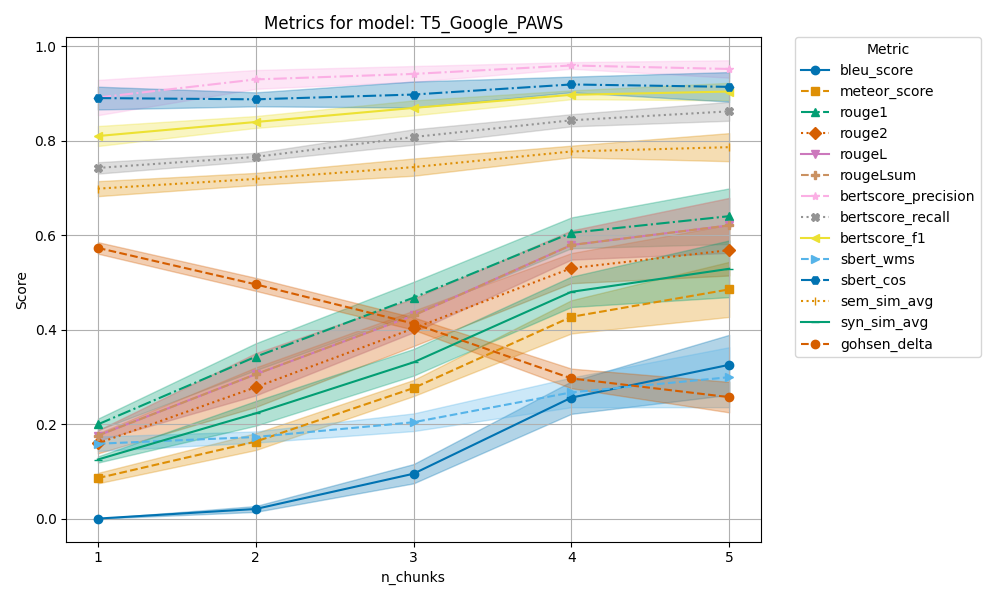
\includegraphics[width=\textwidth]{images/paraphrasing/experiments/T5_Google_PAWS_metrics_plot.png}
    \caption{Average score over different prompts (standard deviation shaded) for different paraphrasing scores for the \ac{t5} model.
    The syntactic scores rise with the number of chunks, while the semantic scores is stable.
    Consequently, the Gohsen Delta score is decreasing with the number of chunks.}
    \label{fig:abl_chunks_T5_Google_PAWS}
\end{figure}

\begin{figure}[htbp]
    \centering
    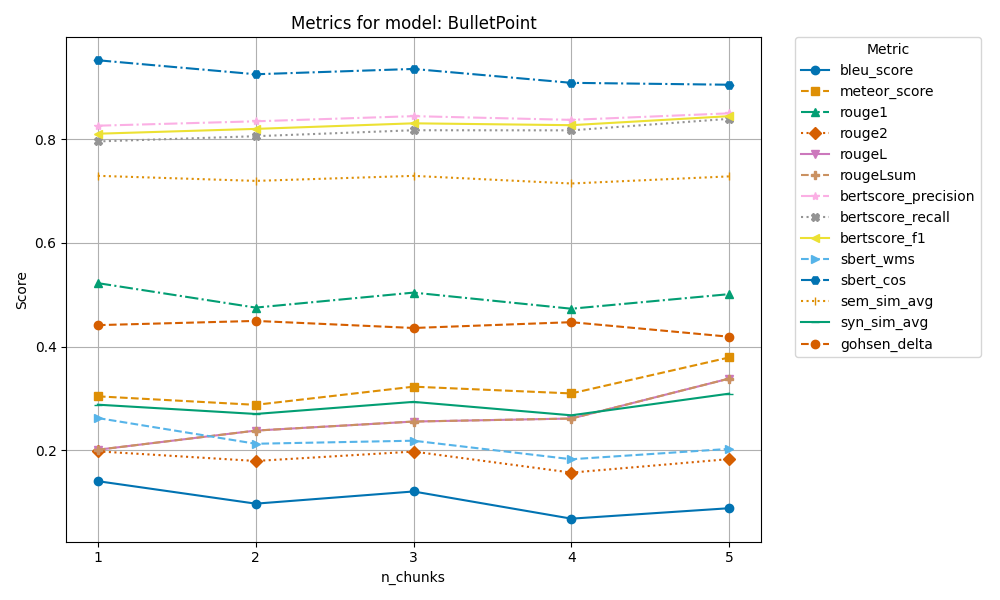
\includegraphics[width=\textwidth]{images/paraphrasing/experiments/BulletPoint_metrics_plot.png}
    \caption{Different paraphrasing scores for the BulletPoint model. 
    This model is not affected by the number of chunks.}
    \label{fig:abl_chunks_BulletPoint}
\end{figure}